\documentclass[10pt,a4paper]{article}
\usepackage[margin=2.2cm]{geometry}
\usepackage{fontspec}
\usepackage{kotex}
\setmainfont{Apple SD Gothic Neo}
\setsansfont{Apple SD Gothic Neo}
\usepackage{amsmath,amssymb}
\usepackage{graphicx}
\usepackage{booktabs}
\usepackage{caption}
\usepackage[dvipsnames]{xcolor}
\usepackage[colorlinks=true,linkcolor=MidnightBlue,citecolor=MidnightBlue,
            urlcolor=MidnightBlue]{hyperref}
\usepackage{titlesec}
\titleformat{\section}{\large\bfseries}{\thesection}{0.6em}{}
\titleformat{\subsection}{\normalsize\bfseries}{\thesubsection}{0.5em}{}
\captionsetup{font=small,labelfont=bf}
\setlength{\parskip}{0.35em}
\setlength{\parindent}{0pt}

\usepackage{mdframed}
\newmdenv[linewidth=0.4pt,linecolor=gray!60,backgroundcolor=gray!5,
          innertopmargin=6pt,innerbottommargin=6pt,skipabove=8pt,skipbelow=8pt]{claimbox}
\newcommand{\claim}[2]{\begin{claimbox}\textbf{주장.} #1\par\smallskip
  \textcolor{gray!70}{\textbf{반증 조건.} #2}\end{claimbox}}

\title{\bfseries 문을 세어 닫고,\\[2pt]
\large 잴 수 있는 것을 찾아 연다}
\author{월드모델 실험실 · 노트 679 · 680}
\date{2026-08-06}
\begin{document}\maketitle

\section{한 줄}

일곱 트랙 중 셋이 ``사람이 KOPIS 를 신청해야 한다''에 묶여 있었다. 그것이 정말
유일한 길인지 한 번도 안 쟀으므로 \textbf{문 넷을 다 두드려 닫았다}. 그리고 그
확정이 새 문제를 만든다 --- T1 이 \emph{무한정} 대기하게 된다. 그래서 T1 에서
\textbf{행이 안 늘어도 잴 수 있는 것}을 찾아 쟀다: \textbf{판의 신호가 텍스트에
있나}. 답은 챔피언의 \textbf{51\%}다.

\section{왜 이 둘이 한 논문인가}

이 실험실이 반복해서 얻은 값이 \emph{``닫은 것을 닫았다고 적는 것''}이다(노트 667 이
팝업 채굴을, 674 가 방문자 축 확장을 그렇게 닫았다). 그런데 닫기만 하면 트랙이
말라 죽는다. \textbf{닫는 행위와 여는 행위는 같은 사이클에 있어야 한다} --- 이 논문의
방법이 그것이다.

\section{닫기 --- 문 넷과 대조 하나}

\begin{figure}[t]\centering
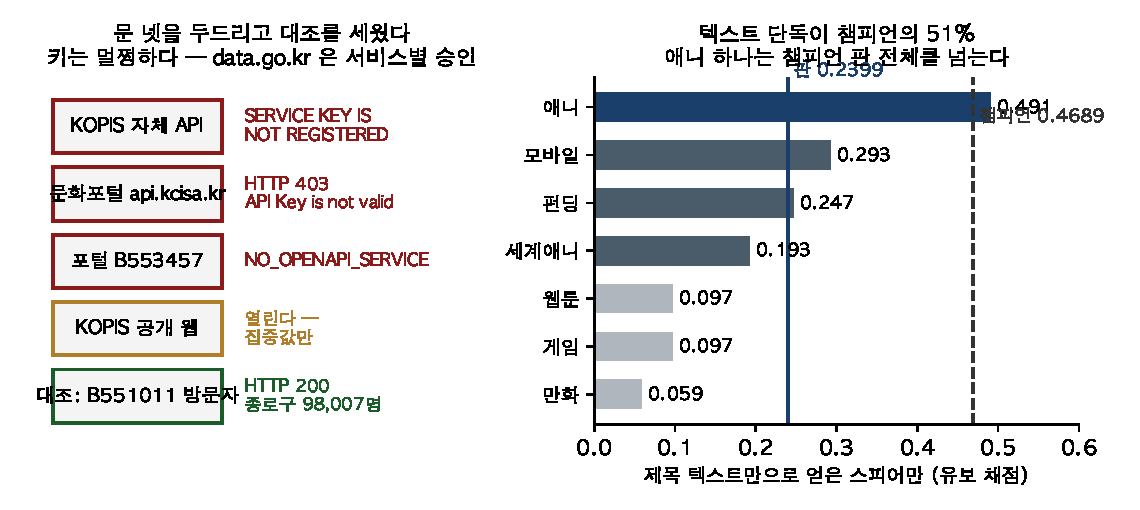
\includegraphics[width=0.99\textwidth]{figs/doors.pdf}
\caption{왼쪽: KOPIS 자체 API 는 \textbf{자체 서비스키}를 요구하고, 문화포털은 403,
공공데이터포털 B553457 은 \texttt{NO\_OPENAPI\_SERVICE}, KOPIS 공개 웹은 열리지만
\textbf{시장 전체 집계}만 있다(2026 상반기 공연 10{,}658건 · 티켓 1{,}141만 매 ·
8{,}095억원). 오른쪽: 텍스트 단독 성적.}
\end{figure}

\claim{공연별 관객수 라벨은 \textbf{사람 승인 없이 얻을 수 없다.} 라벨 있는 행을
\textbf{0건} 얻었다. 눌러야 하는 것은 정확히 하나 --- \texttt{kopis.or.kr} 오픈API
활용신청이다. \textbf{data.go.kr 키는 재발급이 필요 없다}(같은 계정에서 서비스만
추가 신청하면 지금 키가 쓰인다).}
{KOPIS 가 무인증 엔드포인트를 새로 열거나, 제3자가 공연별 관객수를 재배포하면
이 주장이 무너진다. 지금 확인한 문은 넷이고 \textbf{그 넷이 전부라고는 주장하지
않는다.}}

\subsection*{대조가 없었으면 반대로 적었을 것이다}

세 번째 문(\verb|NO_OPENAPI_SERVICE|)을 처음 보고 ``서비스가 폐기됐다''로 읽었다.
그런데 \textbf{대조를 안 세웠다.} 그래서 \verb|ingest/visitors| 의 \emph{되는 것으로
확인된} 경로를 \textbf{같은 키 · 같은 헤더}로 불렀다.

\begin{center}
HTTP \textbf{200} · 종로구 현지인 \textbf{98{,}007명} · \verb|totalCount| 792
\end{center}

키는 멀쩡하다. 그러므로 세 번째 문의 뜻은 \textbf{``data.go.kr 은 서비스별로
승인된다''}이고 우리는 관광(B551011)만 신청했다는 것이다.

\claim{\textbf{실패를 해석하기 전에 성공하는 호출을 하나 세운다.} 대조가 없으면
같은 응답이 ``키가 죽었다''와 ``이 서비스만 안 된다''를 구분하지 못한다 --- 그리고 두
읽기의 처방이 정반대다(키 재발급 대 서비스 추가 신청).}
{되는 경로가 하나도 없는 원천에서는 이 방법이 안 쓰인다. 그때는 응답 코드의
의미를 문서로 확인해야 하고, 문서는 이 실험실이 두 번 틀렸던 근거다(노트 637·639).}

\section{열기 --- 행이 안 늘어도 잴 수 있는 것}

T1\_모델의 물음은 \emph{``어떤 모델을 쓰나 --- 파인튜닝하나, 안 하나''}이고 상태가 두 해
동안 \textbf{막힘}이었다. 사유는 \emph{``T4 가 행을 늘리기 전까지 대기''}. 그런데
방금 T4 를 사람 승인으로 확정했으므로 그 대기가 무한정이 된다.

그래서 물음을 바꿨다. \textbf{언어모델을 파인튜닝한다는 것은 텍스트를 기질로 쓴다는
뜻이다.} 그러면 행이 안 늘어도 물을 수 있는 것이 있다 --- \emph{우리 판의 신호가
텍스트에 있나, 표 형식 축에 있나.}

제목 문자열을 문자 $n$-gram TF-IDF(2$\sim$4자)로 벡터화하고 능형회귀로 라벨 순위를
예측했다. \textbf{학습 구간에서만 적합하고 유보에서 채점}했고(노트 568), \textbf{도메인
안에서만} 했다(제목 길이 · 언어가 도메인 지시자가 되는 것을 막는다).

\begin{center}
\begin{tabular}{lr}
\toprule
& 텍스트만 $\rho$ \\
\midrule
애니 & \textbf{0.4910} \\
모바일 & 0.2928 \\
펀딩 & 0.2469 \\
세계애니 & 0.1927 \\
웹툰 · 게임 & 0.097 \\
만화 & 0.0590 \\
\midrule
\textbf{판}(유보 가중 · 7 도메인 2{,}962행) & \textbf{0.2399} \\
챔피언(11 도메인 3{,}369행) & 0.4689 \\
\bottomrule
\end{tabular}
\end{center}

사전등록 규칙 ②(0.10$\sim$0.30)가 발동한다 --- \textbf{하이브리드만 후보이고
파인튜닝은 아니다.} 예측이 맞았다.

\subsection*{누출 검사를 실제로 했다}

사전등록에 \emph{``판정이 양성이면 상위 $n$-gram 을 눈으로 보고 사후 정보인지
확인한다''}를 적었고, 했다. 애니의 최상위가 \textbf{\texttt{' 1기'}} 이고 음수 쪽이
\texttt{'2 '} · \texttt{'5 '} 다 --- 모형이 \textbf{시즌 번호}를 배웠다.

시간 게이트 위반은 아니다(1기/2기는 방영 전에 정해진다). 그런데 \textbf{2기가 있다는
것은 1기가 성공했다는 뜻}이므로 이것은 \textbf{엔티티 이력의 대용물}이고, 챔피언에는
이미 \texttt{ip\_history.prior\_count} 가 있다.

\claim{텍스트 신호의 상당 부분이 \textbf{기존 축과 겹칠} 수 있다. 그러므로 T1 의
진짜 물음은 ``텍스트가 얼마나 맞히나''가 아니라 \textbf{``텍스트가 챔피언 축 위에
무엇을 더하나''}다. 노트 675 가 관문 ③ 을 \textbf{용량 함수}로 세웠으므로
(겹침 $\leftrightarrow$ 신호 몫 스피어만 $-1.000$) \textbf{그 증분을 재기 전에
예측을 적을 수 있다.}}
{겹침을 재 보니 낮으면 이 주장이 약해지고 텍스트는 새 정보다. 그것이 다음 실험이다.}

\section{정직한 한계}

\begin{itemize}
\item \textbf{TF-IDF 는 언어모델보다 훨씬 약하다.} 그러므로 $0.2399$ 는 \textbf{하한}
      이고, 규칙 ③(0.10 미만)이 나왔더라도 ``언어모델도 못 한다''로는 못 읽는다 ---
      그것을 사전등록에 미리 적었다.
\item \textbf{팝업 계열이 빠졌다}(제목 원천이 없어 판의 88\%만 덮었다). 이 논문을
      쓰는 사이에 세 원천을 찾아 붙였다 --- 팝업 \verb|intervention.brand_name| ·
      시장팝업 \verb|event_name| · 아이돌 \verb|group_name|, 덮음 $0.907$ · $1.000$ ·
      $1.000$. \textbf{다시 재면 숫자가 바뀌고, 7 도메인 판과 11 도메인 판을 견주지
      않는다.}
\item 문 넷이 \textbf{전부라고는 주장하지 않는다.}
\end{itemize}

\end{document}
